\section{Evaluation}
Using the approach from \cref{cha:studydesign}, we now evaluate to what extent the microbenchmark results can predict a change in the application benchmark's results. We divide this section into two subsections. First, we describe the analysis to explain how the findings will be analyzed, and second, we outline the findings and implications of this study. 
\label{cha:evaluation}
\subsection{Analysis}
This research emphasizes two key areas of analysis to evaluate performance results of both application benchmark and microbenchmark and validate the proposed research question: (1) mean query rate and average execution time as performance metrics, and (2) R-squared and Mean Squared Error (\ac{MSE}) for model evaluation. Together, these sections provide a detailed understanding of how performance evolves across versions and how well the ridge regression model predicts application benchmark results using microbenchmark data.  \\
In order to follow best practices when performing both application and microbenchmarks, this research constantly measures the performance of the \ac{SUT} in pairs, where each benchmark compares two consecutive versions of the \ac{SUT} to capture incremental performance changes and reduce the probability of noise affecting the performance measurements. Therefore, each version was compared to its predecessor in all our experiments to evaluate performance changes over time. Specifically, as shown in \cref{tab:compared_versions}, we compared versions v1.104-v1.105, v1.105-v1.106, v1.106-v1.107, v1.107-v1.108 and v1.108-v1.109. This research considers this approach to maintain the reliability of performance comparisons across experiments. Thus, this approach allows us to assess performance shifts, leading to the identification of regressions or optimizations perceived across the compared pair of versions. \\
However, a challenge with this approach is that the bigger the difference between the pair of versions, the greater the chance that the number of common microbenchmarks will be reduced. This challenge is because future versions expect to include code changes that add and remove benchmarks that no longer apply to the newest release. For instance, it is not the same if we compare v1.104 with v1.107 because v1.104 may lack benchmarks that were added in v1.107, resulting in fewer comparable data points; hence, the number of common microbenchmarks between them is less than the common ones that the pair of versions of v1.106 and v1.107 have. Thus, comparing versions using the adjacent version provides us with more reliable and accurate results as it maintains a more significant amount of common microbenchmarks while minimizing noise and ensures that the performance difference can be attributed to the actual effect a code change has on the microbenchmark rather than environmental noise. 
\begin{table}[ht]
    \centering
    \begin{tabular}{c c c} % Bold headers
        \toprule
        \textbf{Version 1} & \textbf{Version 2} \\
        \midrule
        v1.104 & v1.105 \\
        v1.105 & v1.106 \\
        v1.106 & v1.107 \\
        v1.107 & v1.108 \\
        v1.108 & v1.109 \\
        \bottomrule
    \end{tabular}
    \caption{Pair of SUT versions compared}
    \label{tab:compared_versions}
\end{table}

\subsubsection{Performance metrics}
This research analyzes two performance metrics to measure the average time required to complete an operation. It calculates the mean query rate in the application benchmark and the average execution time for the microbenchmark. These performance metrics reflect how the system behaves and responds under load and how external conditions influence it by capturing overall performance trends, including occasional highs or lows. \\
This research aims to identify performance trends using the mean query rate and the average execution time of each pair of versions. Those values are passed to the ridge regression model to perform the prediction. Nevertheless, these metrics have a limitation, as they are calculated using averages; they are sensitive to outliers; thus, they must be considered correctly to avoid distorting performance measurements. However, ridge regression addresses this limitation by applying L2 regularization, which prevents the model from overfitting to outliers, smoothing the impact on high and low values, and allowing the model to learn general performance patterns while keeping away the external noise. Therefore, this regularization allows the model to consider both the mean and the outliers without overfitting the model. \\
The mean query rate and the average execution time metrics help us identify patterns to predict whether a new code version will lead to performance improvements or degradation. A decrease in these two metrics indicates optimization and faster execution times, whereas an increase may suggest performance regression.  

\subsubsection{R-Squared and MSE}
This research considers two main values, the R-squared and the mean square error (\ac{MSE}), to determine how well the ridge regression model performed \cite{mcdonald2009ridgeregression, chicco2021coefficientofdetermination, wang2009meansquareerror}. These metrics provide insights into the model’s ability to fit and predict data, helping assess prediction accuracy. The R-squared explains the proportion of the variance of the input features and performance seen in the model. Its value ranges between 0 and 1; the closer it gets to 1, the better the model fits \cite{chicco2021coefficientofdetermination}. In this analysis, a high R-squared value indicates that the model successfully captures the relationship between the versions changed and the performance output, indicating that the model successfully reflects performance trends influenced by code changes between versions. \\
However, the R-squared alone does not guarantee a good model performance; the \ac{MSE} must be considered. The \ac{MSE} calculates the average squared differences between predicted and actual values. Lower \ac{MSE} values are desirable, opposite to the R-squared. The lower the \ac{MSE}, the better the model, which indicates better prediction accuracy as it shows that the model’s predictions are closer to the actual values \cite{wang2009meansquareerror}. \\
Evaluating these two parameters together helps distinguish between overfitting and underfitting. It allows us to balance fit and generalization used in the training and test sets by explaining sufficient variance without incurring high prediction errors on unseen data by the model.  \\
Having a high R-squared and a low \ac{MSE} in the training set but a high \ac{MSE} in the test set makes the model overfitting. Overfitting means the model performs well during the training set but poorly in the testing set. \\
Overfitting suggests that the model memorizes training data instead of learning general trends. On the contrary, low R-squared and high \ac{MSE} on both the training and test sets make the model underfitting. Underfitting means the model performs poorly in training and test sets, suggesting it cannot capture the data complexity. \\
This research aims to portray a balanced ridge regression that is neither overfitting nor underfitting. The R-squared and \ac{MSE} values demonstrate that the model generalizes well across training and testing sets, indicating that it has learned performance patterns without relying on specific data. Making the model more robust to provide insightful performance predictions.


\subsection{Findings and Implications}
\label{cha:results}
This section presents the results obtained from the experiments and has the following subsections. First, we analyze the results obtained by the application benchmark, where we detect performance changes in the application environment. Second, we analyze the microbenchmark's results to determine how accurately the performance changes in microbenchmarks affect the performance prediction of the application benchmark suites. Finally, this research further analyzes the findings and implications, combining the application benchmarks and microbenchmark's results into the ridge regression model and how well the model performed before analyzing the individual results of both the application and microbenchmark. This research needs to verify that two things are successfully achieved to ensure accurate and reliable results: First, we must ensure that the \ac{SUT} is fully stressed before we analyze the results in both the application and microbenchmarks. 

\begin{figure}[!htbp]
    \captionsetup[subfigure]{list=true}
     \centering
     \begin{subfigure}[b]{0.7\textwidth}
         \centering
         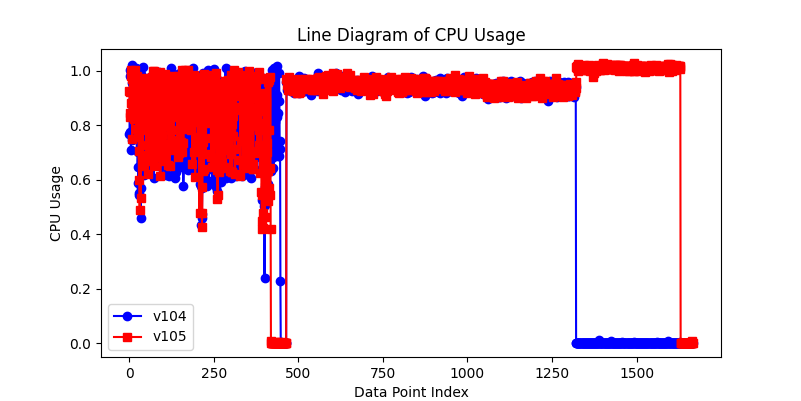
\includegraphics[width=\textwidth]{figures/applicationBenchmark_SUT.png}
         \caption{Application Benchmark}
         \label{fig:applicationBenchmark_SUT}
     \end{subfigure}
     \hfill
     \begin{subfigure}[b]{0.7\textwidth}
         \centering
         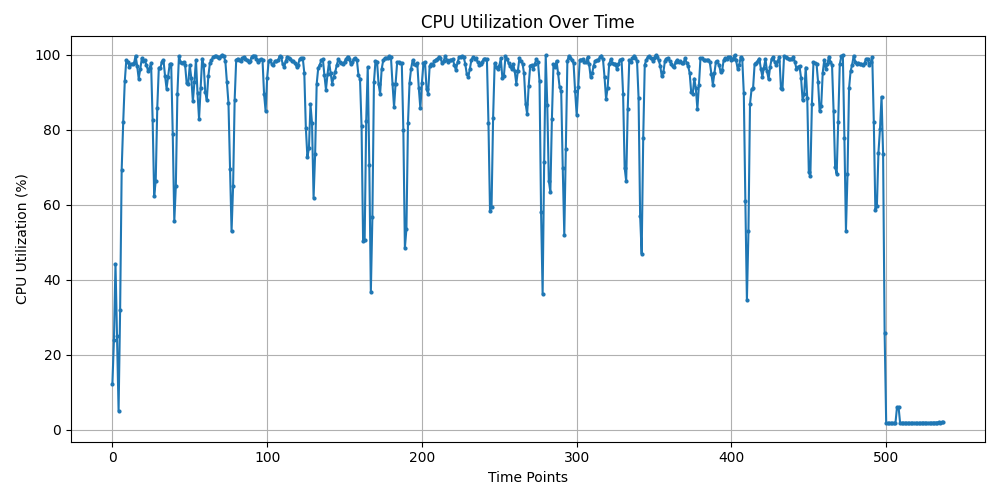
\includegraphics[width=\textwidth]{figures/cpu_utilization_analysis.png}
         \caption{Microbenchmark}
         \label{fig:microbenchmark_SUT}
     \end{subfigure}
     \caption{SUT under stress}
     \label{fig:SUT_under_streess}
\end{figure}

\cref{fig:SUT_under_streess} shows the \ac{SUT} of the application benchmark and the microbenchmark. Both show the \ac{SUT} as fully stressed. Second, we must verify that the application logs were completed successfully without errors. Ensuring this guarantees that the data was loaded successfully and that all the queries were run. 

\subsubsection{Application benchmark}
The application benchmark experiments required approximately 1.5 hours per run, split into two main phases: data insertion and Group-by query execution. The first phase is loading the 581.760.000 metrics into the  \ac{SUT}; this phase takes around 45 minutes to complete. The second phase executes the 8640 Group-By queries shown in \cref{tab:applicationBenchmarkParameters} in the system; it takes around 45 minutes to complete. This experiment successfully executes 50 application benchmarks, each pair of versions having 10 experiment runs. For application benchmarks, we compare the same pair of versions mentioned before in \cref{tab:compared_versions}: v1.104-v1.105, v1.105-v1.106, v1.106-v1.107, v1.107-v1.108, and v1.108-v1.109. \\
As application benchmarks have two phases, we have two metrics, one per phase. First, we have the mean insertion time for inserting the data into the \ac{SUT}, which refers to the first phase. Second, we have the mean query rate for executing all the Group-By queries in the second phase. The mean insertion time explains how much time, on average, each version of the application benchmark requires to insert 581.760.000 metrics, 51.840.000 rows, and 691.200 queries into the \ac{SUT}. \cref{fig:mean_inserts_time_all_runs-v104-v105,fig:mean_inserts_time_all_runs-v105-v106,fig:mean_inserts_time_all_runs-v106-v107,fig:mean_inserts_time_all_runs-v107-v108,fig:mean_inserts_time_all_runs-v108-v109} illustrate the variance in the mean insertion time during the data insertion phase across the 10 runs for each pair of versions v1.104-v1.105, v1.105-v1.106, v1.106-v1.107, v1.107-v1.108, and v1.108-v1.109, respectively.

\begin{figure}[ht]
    \captionsetup[subfigure]{list=true}
    \centering
    % -- Row 1: two subfigures --
    \begin{subfigure}[b]{0.48\textwidth}
        \centering
        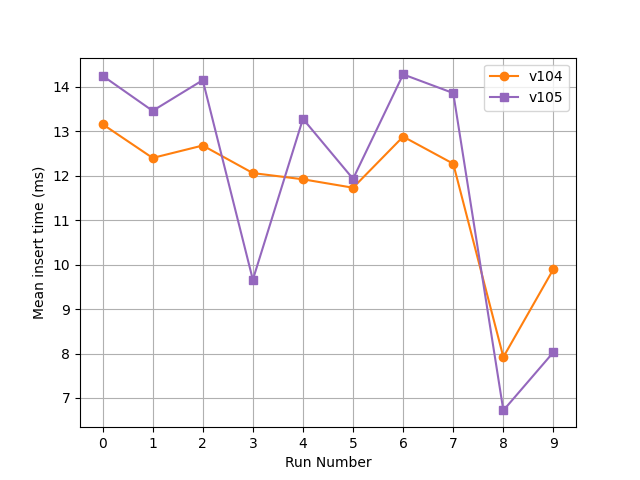
\includegraphics[width=\textwidth]{figures/mean_inserts_time_all_runs-v104-v105.png}
        \caption{v1.104--v1.105}
        \label{fig:mean_inserts_time_all_runs-v104-v105}
    \end{subfigure}
    \hfill
    \begin{subfigure}[b]{0.48\textwidth}
        \centering
        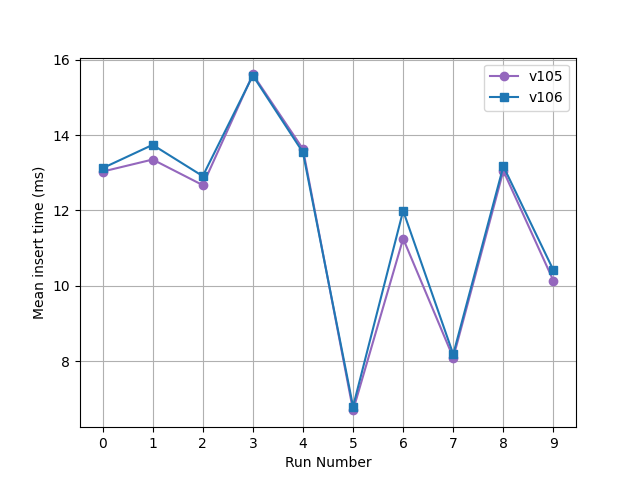
\includegraphics[width=\textwidth]{figures/mean_inserts_time_all_runs-v105-v106.png}
        \caption{v1.105--v1.106}
        \label{fig:mean_inserts_time_all_runs-v105-v106}
    \end{subfigure}

    \vskip\baselineskip  % vertical space between rows

    % -- Row 2: two subfigures --
    \begin{subfigure}[b]{0.48\textwidth}
        \centering
        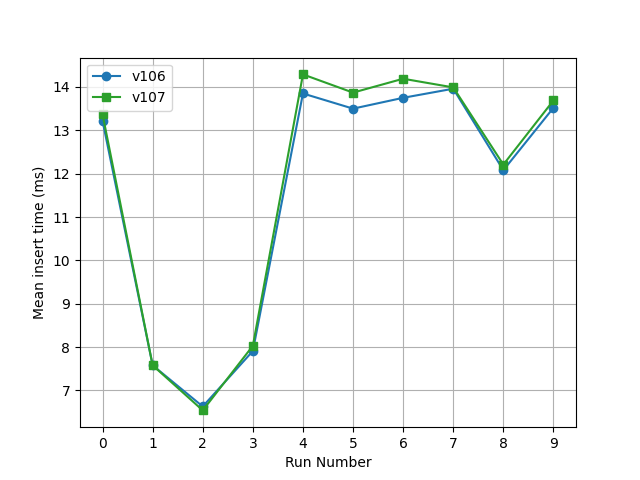
\includegraphics[width=\textwidth]{figures/mean_inserts_time_all_runs-v106-v107.png}
        \caption{v1.106--v1.107}
        \label{fig:mean_inserts_time_all_runs-v106-v107}
    \end{subfigure}
    \hfill
    \begin{subfigure}[b]{0.48\textwidth}
        \centering
        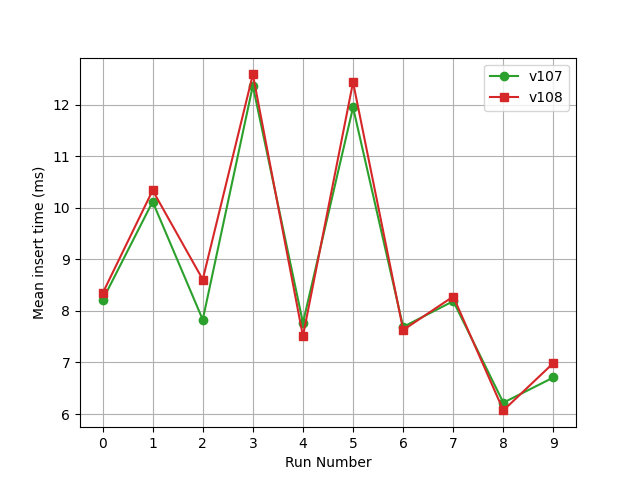
\includegraphics[width=\textwidth]{figures/mean_inserts_time_all_runs-v107-v108.png}
        \caption{v1.107--v1.108}
        \label{fig:mean_inserts_time_all_runs-v107-v108}
    \end{subfigure}

    \vskip\baselineskip  % vertical space between rows

    % -- Row 3: single subfigure --
    \begin{subfigure}[b]{0.48\textwidth}
        \centering
        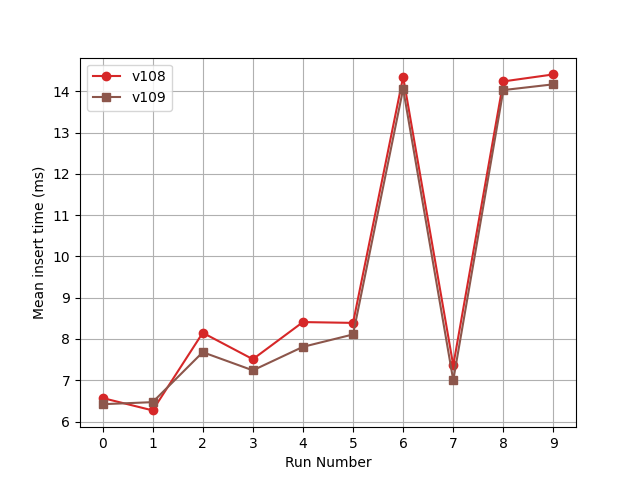
\includegraphics[width=\textwidth]{figures/mean_inserts_time_all_runs-v108-v109.png}
        \caption{v1.108--v1.109}
        \label{fig:mean_inserts_time_all_runs-v108-v109}
    \end{subfigure}

    \caption{Insert time}
    \label{fig:insertTime}
\end{figure}



\begin{figure}[ht]
    \captionsetup[subfigure]{list=true}
    \centering
    % -- Row 1: two subfigures --
    \begin{subfigure}[b]{0.48\textwidth}
        \centering
        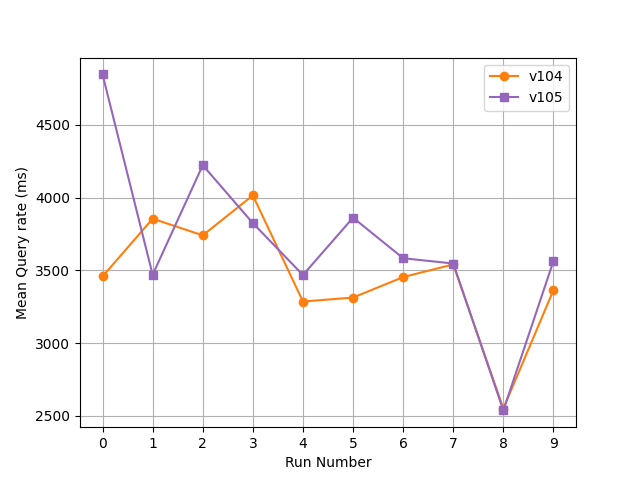
\includegraphics[width=\textwidth]{figures/mean_query_rate_all_runs-v104-v105.png}
        \caption{v1.104--v1.105}
        \label{fig:mean_query_rate_all_runs-v104-v105}
    \end{subfigure}
    \hfill
    \begin{subfigure}[b]{0.48\textwidth}
        \centering
        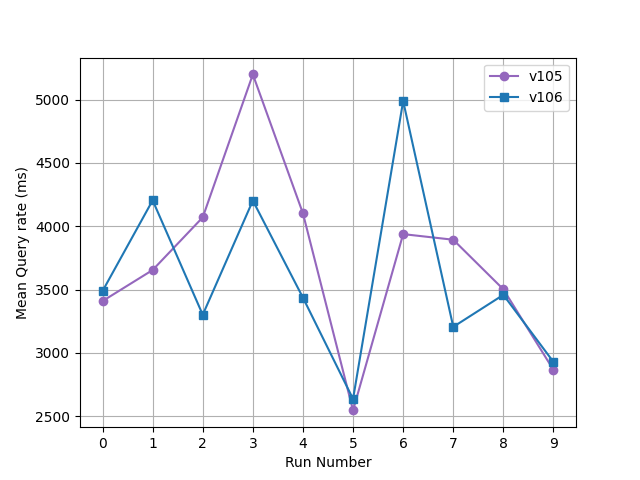
\includegraphics[width=\textwidth]{figures/mean_query_rate_all_runs-v105-v106.png}
        \caption{v1.105--v1.106}
        \label{fig:mean_query_rate_all_runs-v105-v106}
    \end{subfigure}

    \vskip\baselineskip  % vertical space between rows

    % -- Row 2: two subfigures --
    \begin{subfigure}[b]{0.48\textwidth}
        \centering
        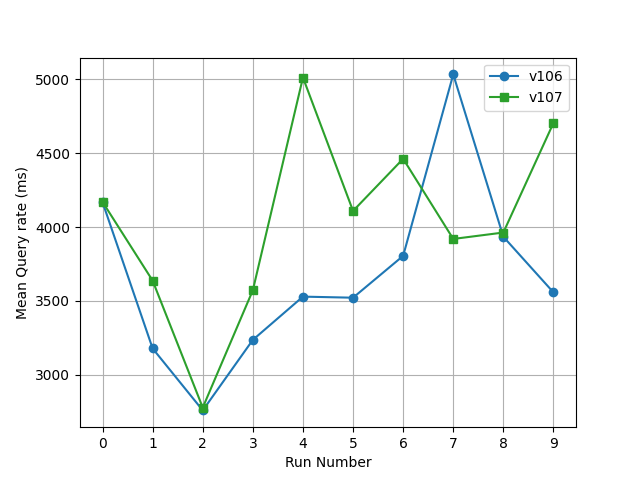
\includegraphics[width=\textwidth]{figures/mean_query_rate_all_runs-v106-v107.png}
        \caption{v1.106--v1.107}
        \label{fig:mean_query_rate_all_runs-v106-v107}
    \end{subfigure}
    \hfill
    \begin{subfigure}[b]{0.48\textwidth}
        \centering
        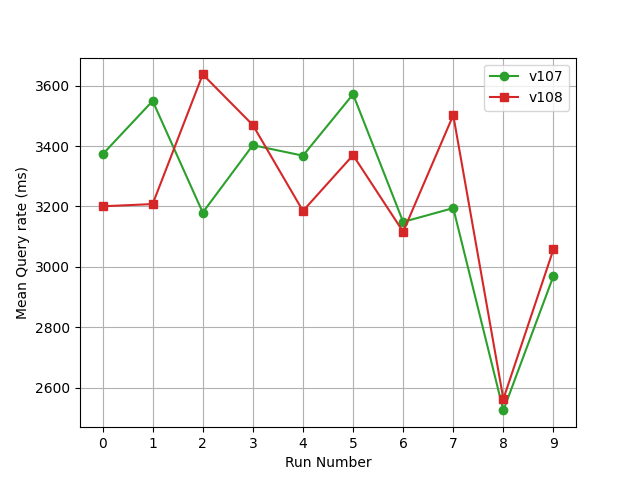
\includegraphics[width=\textwidth]{figures/mean_query_rate_all_runs-v107-v108.png}
        \caption{v1.107--v1.108}
        \label{fig:mean_query_rate_all_runs-v107-v108}
    \end{subfigure}

    \vskip\baselineskip  % vertical space between rows

    % -- Row 3: single subfigure --
    \begin{subfigure}[b]{0.48\textwidth}
        \centering
        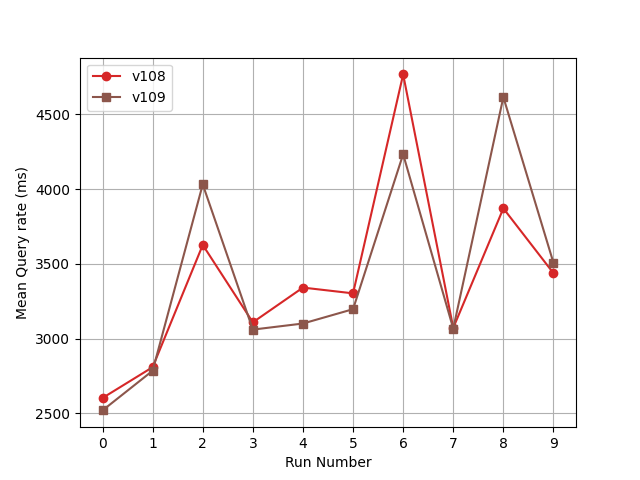
\includegraphics[width=\textwidth]{figures/mean_query_rate_all_runs-v108-v109.png}
        \caption{v1.108--v1.109}
        \label{fig:mean_query_rate_all_runs-v108-v109}
    \end{subfigure}

    \caption{Mean query rate for various version intervals.}
    \label{fig:mean_query_rate}
\end{figure}

\cref{fig:mean_inserts_time_all_runs-v104-v105,fig:mean_inserts_time_all_runs-v106-v107,fig:mean_inserts_time_all_runs-v105-v106,fig:mean_inserts_time_all_runs-v107-v108,fig:mean_inserts_time_all_runs-v108-v109}, show that the performance of each pair of versions is stable, ranging from 6 \ac{ms} to a maximum of 16 \ac{ms}. \cref{fig:mean_inserts_time_all_runs-v104-v105} portrays the biggest variation in the mean insert values between both versions. Meanwhile, \cref{fig:mean_inserts_time_all_runs-v105-v106,fig:mean_inserts_time_all_runs-v106-v107,fig:mean_inserts_time_all_runs-v107-v108,fig:mean_inserts_time_all_runs-v108-v109} show that both versions in each pair follow the same trend and have less variance between them.\\
Furthermore, the mean query rate of executing all the Group-By queries explains how much time, on average, each version of the application benchmarks requires to execute the 8640 group-by queries successfully.  \cref{fig:mean_query_rate} shows the variance of the mean query rate of executing all the Group-By queries over the 10 runs of the pair versions v1.104-v1.105, v1.105-v1.106, v1.106-v1.107, v1.107-v1.108 and v1.108-v1.109.  \\
As seen in  \cref{fig:mean_query_rate_all_runs-v104-v105,fig:mean_query_rate_all_runs-v105-v106,fig:mean_query_rate_all_runs-v106-v107,fig:mean_query_rate_all_runs-v107-v108,fig:mean_query_rate_all_runs-v108-v109},  the variance of the mean query rate of the pair versions was consistent, ranging from 2500 \ac{ms} to 5000 \ac{ms}. \cref{fig:mean_query_rate_all_runs-v107-v108} shows that the pair of versions with less variance was v1.107-v1.108, where the maximum value was 3600 \ac{ms} and the minimum 2500 \ac{ms}, matching the expectation that the newer the version is, the better the performance would be. The variance analysis across both phases helps us determine the consistency and reliability of each version's performance under load. Thus, the following section considers the mean latencies of both phases (data insertion and Group-by queries execution) as the dependent variable in the ridge regression model, as this is the value that the model proposed in this research aims to predict. 

\subsubsection{Microbenchmark}
After running the complete microbenchmark suite, we noticed that each microbenchmark run took around 8 hours to complete due to the setup configuration. \cref{tab:compared_versions} shows this research tested five pairs of versions: v1.104-v1.105, v1.105-v1.106, v1.106-v1.107, v1.107- v1.108 and v1.108-v1.109. Both pairs of versions, v1.104-v1.105 and v1.105-v1.106, were executed with 552 microbenchmarks, and versions v1.106-v1.107 and v1.107-v1.108 executed a total of 549 microbenchmarks, whereas version v1.108-v1.109 executed a total of 546 microbenchmarks. Confirming the assumption that as the software evolves over multiple versions, the greater the distance between one version and the other, the fewer common features will be present in both microbenchmarks’ versions. \\
Additionally, we noticed that the results do not contain a mean metric for the 10 runs executed; we had to perform a step where we got all the data from the different runs of the experiments to calculate the mean execution time metric by ourselves. In this step, we used Python to perform all the data transformations, specifically using libraries like numpy and Pandas. As a result, we calculated the mean for the three runs and five iterations, which gave 45 measurements for each of the microbenchmarks executed on each version. We sum this value with the other nine executions and divide by the number of runs (10), and that is how we calculate the mean of the microbenchmarks that help us clean up the model's data.  \\
Then, we proceeded to perform a collinearity analysis to improve the feature selection for the model, which allowed us to optimize the set of microbenchmarks provided to the model by eliminating the high collinearity between the microbenchmark's functions and removing redundant features. As a result, we will use a subset of microbenchmarks in the ridge regression model to make predictions of the application benchmark performance. \\
However, the model will be accurate and valuable only if it guarantees that the same subset of microbenchmarks will always be present in future versions. Otherwise, the non-present microbenchmarks will be replaced by 0 to avoid including invalid data that leads to wrong predictions. The mean execution time for each microbenchmark, calculated in \ac{ms}, provides insight into performance differences across versions. This metric helps us evaluate performance changes between the pair of versions in the  \ac{SUT}. \cref{tab:version_time} summarizes the mean execution time of each pair of versions. By comparing the mean execution time across versions, we can determine if its performance has improved or degraded. When comparing both versions, if the mean execution time increases, it may indicate a performance regression as it takes more time to execute the microbenchmark. On the contrary, if the mean execution time decreases, the performance improves, suggesting that the function is optimized, providing a faster execution time. Therefore, this comparison allows us to identify the performance impact that code changes have across the pair versions.  \\
\cref{tab:version_time} illustrates that the mean execution time in minutes between v1.104 and v1.105 is 488,489, the one for v1.105-v1.106 is 493,455, v1.106-v1.107 is 490,523, v1.107-v1.108 is 482,036, and v1.108-v1.109 is 484,105. These results show that the mean execution time between versions v1.104-v1.105 is lower than the pair of versions v1.105-v1.106 and v1.106-v1.107. On the other hand, the mean execution time between v1.107-v1.108 and v1.108-v1.109 is lower than the mean execution time of the pair version v1.104-v1.105. Therefore, \cref{tab:version_time} suggests that the performance in the pair version v1.104-v1.105 was better than the subsequent versions, meaning that v1.105-v1.106 and v1.106-v1.107 required more time to be successfully executed on average, which implies that the performance degraded in these two pair versions. Additionally, the performance of versions v1.107-v1.108 and v1.108-v1.109 improved, showing that they both required less time to complete than versions v1.104-v1.105. The increase and decrease in the mean execution time between these pair versions might be attributed to code changes or features implemented in the newer versions, affecting their performance. After performing the 10 runs for each pair of versions, each run will have the average execution time for each microbenchmark. The following section will use these results in our ridge regression model to help capture performance behavior and predict future performance trends.  

\begin{table}[ht]
    \centering
    
    \begin{tabular}{c c c} % Bold headers
        \toprule
        \textbf{Version} & \textbf{Minutes} & \textbf{Hours} \\
        \midrule
        v1.104 - v1.105 & 488.879 & 8.147 \\
        v1.105 - v1.106 & 493.455 & 8.224 \\
        v1.106 - v1.107 & 490.523 & 8.175 \\
        v1.107 - v1.108 & 482.036 & 8.033 \\
        v1.108 - v1.109 & 484.105 & 8.068 \\
        \bottomrule
    \end{tabular}
    \caption{Time Comparison Between Versions}
    \label{tab:version_time}
\end{table}


\subsubsection{Ridge regression Model}
Before we could use the data generated by the microbenchmarks and application benchmark in the ridge regression model, we noticed that the distribution of our data was not as linear as expected. Therefore, further analyses were conducted to improve the model's feature selection. We do an optimization that, in this case, was a pre-clean-up step for the data, where, with the help of a correlation matrix, we performed the feature selection step to determine how much the features were collinear with each other; this helped us reduce the number of microbenchmarks used as features in the model. \\
The ridge regression model uses the average execution time from the microbenchmarks as features and the mean query rate as the target variable. Then, the R-squared and \ac{MSE} metrics are calculated to indicate the model's accuracy.  \\
\cref{tab:threshold_metrics} shows the results of the threshold, features, R-squared, and \ac{MSE}. The threshold is the alpha parameter the ridge regression takes as an input to penalize the features to avoid overfitting the model. The features refer to the number of microbenchmarks used to train the model. R-squared and \ac{MSE} determine how good the model is.  \\
\cref{tab:threshold_metrics} that different thresholds were implemented with different amounts of features to analyze the changes in both R-squared and \ac{MSE}. However, due to the microbenchmarks' high collinearity, it was impossible to identify an alpha value that could explain how data was distributed, giving us a high R-squared and low \ac{MSE}. The results show that this model has a low R-squared and high \ac{MSE}, which means that the model presents overfitting. 

\begin{table}[ht]
    \centering
    \begin{tabular}{c c c c} % Bold headers
        \toprule
        \textbf{Threshold} & \textbf{Features} & \textbf{MSE} & \textbf{R²} \\
        \midrule
        0.0000100000 &  4   & 424344.5968 & -0.2093 \\
        0.0000010000 & 28   & 349287.0872 &  0.0046 \\
        0.0000001000 & 75   & 349287.0876 &  0.0046 \\
        0.0000000100 & 153  & 349286.7702 &  0.0046 \\
        0.0000000010 & 240  & 349300.2626 &  0.0046 \\
        \bottomrule
    \end{tabular}
    \caption{Performance Metrics at Different Thresholds}
    \label{tab:threshold_metrics}
\end{table}

